\documentclass{beamer}

\newcommand{\week}{Week 1-b}

\title{Financial Market Returns}
\subtitle{Reference: Bodie et al, Ch 5}
\author{Econ 457}
\date{\week}

% Reference the shared preamble
\setbeamertemplate{frametitle}{
  \vspace{0.5em}
  \insertframetitle
  \par
  \vspace{0.5em}
  \hrule
  \vspace{0.3em}
  {\small\color{gray}\insertframesubtitle}
}

\setbeamertemplate{navigation symbols}{}
\setbeamertemplate{itemize item}{\textbullet} % main bullet: filled dot
\setbeamertemplate{itemize subitem}{\normalsize$\circ$} % sub-bullet: empty dot
\setbeamertemplate{itemize subsubitem}{\scriptsize--} % sub-sub-bullet: dash


% Font changes
\usepackage[scaled=0.92]{helvet}
\renewcommand{\familydefault}{\sfdefault}

% Packages
\usepackage{tikz}
\usepackage{booktabs}
\usepackage{xcolor}
\usepackage{array}           % Enhanced column types for tables
\usepackage{multirow}        % Spanning multiple rows in tables
\usepackage{makecell}        % Line breaks and formatting in table cells
\usepackage{siunitx}         % Proper formatting of numbers and units
\usepackage{amsmath}         % Enhanced math environments
\usepackage{amsfonts}        % Additional math fonts
\usepackage{amssymb}         % Additional math symbols
\usepackage{url}             % Better URL formatting
\usepackage{graphicx}        % Enhanced graphics support
\usepackage{tabularray}
\UseTblrLibrary{booktabs, siunitx, varwidth}
% For financial presentations specifically
\usepackage{eurosym}         % Euro symbol
\usepackage{textcomp}        % Additional text symbols
\usepackage{hyperref}        % Hyperlinks (should be loaded last)

% Define a footnote
\renewcommand{\footnoterule}{\vspace*{-3pt}\hrule width 2in height 0.4pt\vspace*{2.6pt}}

% Define a Foundation Slide
\newenvironment{foundframe}[1][t]{
    \setbeamercolor{background canvas}{bg=gray!8}
    \setbeamercolor{frametitle}{fg=gray!80!black,bg=gray!25}
    \setbeamercolor{framesubtitle}{fg=gray!70!black,bg=gray!15}
    \setbeamercolor{item}{fg=gray!80!black}
    \setbeamercolor{enumerate item}{fg=gray!80!black}
    
    % Modify the frametitle template for this frame type
    \setbeamertemplate{frametitle}{
        \vspace{0.5em}
        \begin{minipage}[t]{0.75\textwidth}
            \insertframetitle
            \par
            \vspace{0.5em}
            \hrule
            \vspace{0.3em}
            {\small\color{gray}\insertframesubtitle}
        \end{minipage}%
        \hfill
        \begin{minipage}[t]{0.2\textwidth}
            \raggedleft
            \colorbox{gray!30}{%
                \scriptsize\bfseries\color{gray!80!black}%
                   \hspace{3pt}\begin{tabular}{c}Foundation\\Material\end{tabular}\hspace{3pt}%
            }
        \end{minipage}
        \vspace{0.3em}
    }
    
    \begin{frame}[#1]
}{
    \end{frame}
}

% Define Practice Slide
\newenvironment{practiceframe}[1][t]{
    \setbeamercolor{background canvas}{bg=white}
    \setbeamercolor{frametitle}{fg=blue!80!black,bg=blue!15}
    \setbeamercolor{framesubtitle}{fg=blue!70!black,bg=blue!10}
    \setbeamercolor{item}{fg=blue!80!black}
    \setbeamercolor{enumerate item}{fg=blue!80!black}
    \setbeamercolor{normal text}{fg=blue!90!black}
    
    % Modify the frametitle template for this frame type
    \setbeamertemplate{frametitle}{
        \vspace{0.5em}
        \begin{minipage}[t]{0.75\textwidth}
            \insertframetitle
            \par
            \vspace{0.5em}
            \hrule
            \vspace{0.3em}
            {\small\color{blue!70!black}\insertframesubtitle}
        \end{minipage}%
        \hfill
        \begin{minipage}[t]{0.2\textwidth}
            \raggedleft
            \colorbox{blue!20}{%
                \scriptsize\bfseries\color{blue!80!black}%
                   \hspace{3pt}\begin{tabular}{c}Practice\\Questions\end{tabular}\hspace{3pt}%
            }
        \end{minipage}
        \vspace{0.3em}
    }
    
    \begin{frame}[#1]
}{
    \end{frame}
}

% Define Excel Slide
\newenvironment{excelframe}[1][t]{
    \setbeamercolor{background canvas}{bg=white}
    \setbeamercolor{frametitle}{fg=blue!80!black,bg=blue!15}
    \setbeamercolor{framesubtitle}{fg=blue!70!black,bg=blue!10}
    \setbeamercolor{item}{fg=blue!80!black}
    \setbeamercolor{enumerate item}{fg=blue!80!black}
    \setbeamercolor{normal text}{fg=blue!90!black}
    
    % Modify the frametitle template for this frame type
    \setbeamertemplate{frametitle}{
        \vspace{0.5em}
        \begin{minipage}[t]{0.75\textwidth}
            \insertframetitle
            \par
            \vspace{0.5em}
            \hrule
            \vspace{0.3em}
            {\small\color{blue!70!black}\insertframesubtitle}
        \end{minipage}%
        \hfill
        \begin{minipage}[t]{0.2\textwidth}
            \raggedleft
            \colorbox{green!10}{%
                \scriptsize\bfseries\color{blue!80!black}%
                   \hspace{3pt}\begin{tabular}{c}MS Excel\end{tabular}\hspace{3pt}%
            }
        \end{minipage}
        \vspace{0.3em}
    }
    
    \begin{frame}[#1]
}{
    \end{frame}
}

% Define Caution Slide
\newenvironment{cautionframe}[1][t]{
    \setbeamercolor{background canvas}{bg=white}
    \setbeamercolor{frametitle}{fg=blue!80!black,bg=blue!15}
    \setbeamercolor{framesubtitle}{fg=blue!70!black,bg=blue!10}
    \setbeamercolor{item}{fg=blue!80!black}
    \setbeamercolor{enumerate item}{fg=blue!80!black}
    \setbeamercolor{normal text}{fg=blue!90!black}
    
    % Modify the frametitle template for this frame type
    \setbeamertemplate{frametitle}{
        \vspace{0.5em}
        \begin{minipage}[t]{0.75\textwidth}
            \insertframetitle
            \par
            \vspace{0.5em}
            \hrule
            \vspace{0.3em}
            {\small\color{blue!70!black}\insertframesubtitle}
        \end{minipage}%
        \hfill
        \begin{minipage}[t]{0.2\textwidth}
            \raggedleft
            \colorbox{red!10}{%
                \scriptsize\bfseries\color{blue!80!black}%
                   \hspace{3pt}\begin{tabular}{c}Caution\end{tabular}\hspace{3pt}%
            }
        \end{minipage}
        \vspace{0.3em}
    }
    
    \begin{frame}[#1]
}{
    \end{frame}
}

% Add to footnotes
\makeatletter
\newcommand\blfootnote[1]{%
  \begingroup
  \renewcommand\thefootnote{}%
  \renewcommand\@makefntext[1]{\raggedright\leftskip=0pt ##1}%
  \footnote{\scriptsize #1}%
  \addtocounter{footnote}{-1}%
  \endgroup
}
\makeatother

% Set the footer -- change 
\setbeamertemplate{footline}{
  \leavevmode%
  \vspace{2ex}
  \hbox{%
    % Left box: Econ 457
    \begin{beamercolorbox}[wd=.4\paperwidth,ht=2.5ex,dp=1ex,left]{author in head/foot}%
      \hspace{1em}Econ 457
    \end{beamercolorbox}%
    % Middle box: Week
    \begin{beamercolorbox}[wd=.2\paperwidth,ht=2.5ex,dp=1ex,center]{date in head/foot}%
      \centering\week
    \end{beamercolorbox}%
    % Right box: Slide numbers
    \begin{beamercolorbox}[wd=.4\paperwidth,ht=2.5ex,dp=1ex,center]{date in head/foot}%
      \hfill\insertframenumber{} 
    \end{beamercolorbox}%
  }%
  \vskip0pt%
}

\begin{document}

\frame{\titlepage}

\begin{frame}
    \frametitle{Outline}

    \vspace{2em}

    \begin{enumerate}
        \item Exponentials and Logarithms
        \item Measuring Returns
        \item Income
        \item Measurment Issues: 
        \begin{itemize}
            \item Compounding, Geo v. Arth Mean, Total Return Series
        \end{itemize}
        \item Excel
    \end{enumerate}
\end{frame}

\begin{foundframe}[t]
    \frametitle{1. Exponentials and Logarthims}
    \framesubtitle{Some basic facts}

    Exponential Function:
    $$10^4 = 10 \times 10 \times 10 \times 10$$

    First derivative:
    $$\frac{d(e^x)}{dx} = e^x$$

    Negative Exponents:
    $$a^{-x} = \frac{1}{a^x}$$

    Fractional Exponents:
    $$a^{1/x} = \sqrt[x]{a}$$

\end{foundframe}

\begin{foundframe}[t]
    \frametitle{1. Exponentials and Logarthims}
    \framesubtitle{Some basic facts, cont'd}

    Logarithim is the inverse of the exponential function.  $log_{10}()$ is the inverse of $10^x$ and $ln()$ is the inverse of $e^x$
    \vspace{1em}

    First derivative:
    $$\frac{d(ln(x))}{dx} = \frac{1}{x}$$

    Logarithms of expressions with exponents:\\
    $$log(x^a) = a \cdot log(x)$$

    Logarithm of expressions with products:\\
    $$log(x \cdot y) = log(x) + log(y)$$


\end{foundframe}

\begin{foundframe}[t]
    \frametitle{1. Exponentials and Logarthims}
    \framesubtitle{Some basic facts, cont'd}

    Two more facts about logarthims we are going to use in this lecture:
    \begin{enumerate}
    \item  In a log-linear graph the scale of the y-axis is $log(y)$ or $ln(y)$.  
    The slope of the log-linear graph is the average (continously compounded) growth rate.
    \item Logarithim is a concave function:\\
    $$log((a+b)/2) > (log(a) + log(b))/2$$
    \end{enumerate}

\end{foundframe}


\begin{foundframe}[t]
    \frametitle{1. Exponentials and Logarthims}
    \framesubtitle{Some basic facts, cont'd}

    \centering
    \includegraphics[width=0.8\textwidth]{figures/ch5_1_lnexp.png}

\end{foundframe}


\begin{frame}[t]
    \frametitle{2. Measuring Returns}
    \framesubtitle{Total Return - Definition}

    Total Return: A performance metric that accounts for
    capital gains (i.e. changes in price) and income (e.g. dividends, coupons, etc) 
    paid to the owner of a financial security.\\
    \vspace{1em}   
    Total return is typically expressed as a percentage of the initial price.
    $$
    \text{Total Return} = \frac{\text{Income}}{\text{Initial Price}} + \frac{\text{Change in Price}}{\text{Initial Price}}
    $$
    The first term is sometimes referred to as either the "current yield" or "dividend yield",
     and the second term is referred to as the "capital gain rate."

\end{frame}

\begin{frame}[t]
    \frametitle{2. Measuring returns}
    \framesubtitle{Holding Period Return and Annual Percentage Rate}

    Holding Period Return (HPR):\\
    $$\text{HPR} = r(T) = \frac{\text{Price Increase + Income}}{\text{Initial Price}}$$

    Effective Annual Rate (EAR)\\
    $$\text{EAR} = (1+\text{HPR})^{1/T} - 1$$\\
    \begin{itemize}
        \item Where T is the length of time the investment was held in years\\
        \item Express total return as a \textit{rate} of return over a year\\
        \item Notice this assumes annual compounding\\
        \item T could be positive number, greater than 1 or a fraction
    \end{itemize}

\end{frame}


\begin{frame}[t]
    \frametitle{3. Income}
    \framesubtitle{Types of Income}

    \begin{table}
        \centering
        \caption{Income Sources by Investment Type}
        \begin{tabular}{lll}
            \toprule
            Investment Type & Income Source & Frequency\\
            \midrule
            Bonds & Coupon payments & Semi-annual (usually) \\
            Stocks & Dividends & Quarterly \\
            ETFs & Distributions & Quarterly/Annual \\
            \bottomrule
        \end{tabular}
    \end{table}
    \vspace{1em}
    ETF distributions are often composed of dividends or coupons of the underlying assets, but occassionally will include capital gains as well.

\end{frame}

\begin{frame}[t]
    \frametitle{3. Income}
    \framesubtitle{Treasury Bond: Note the ``coupons'' at the bottom}
    \centering
    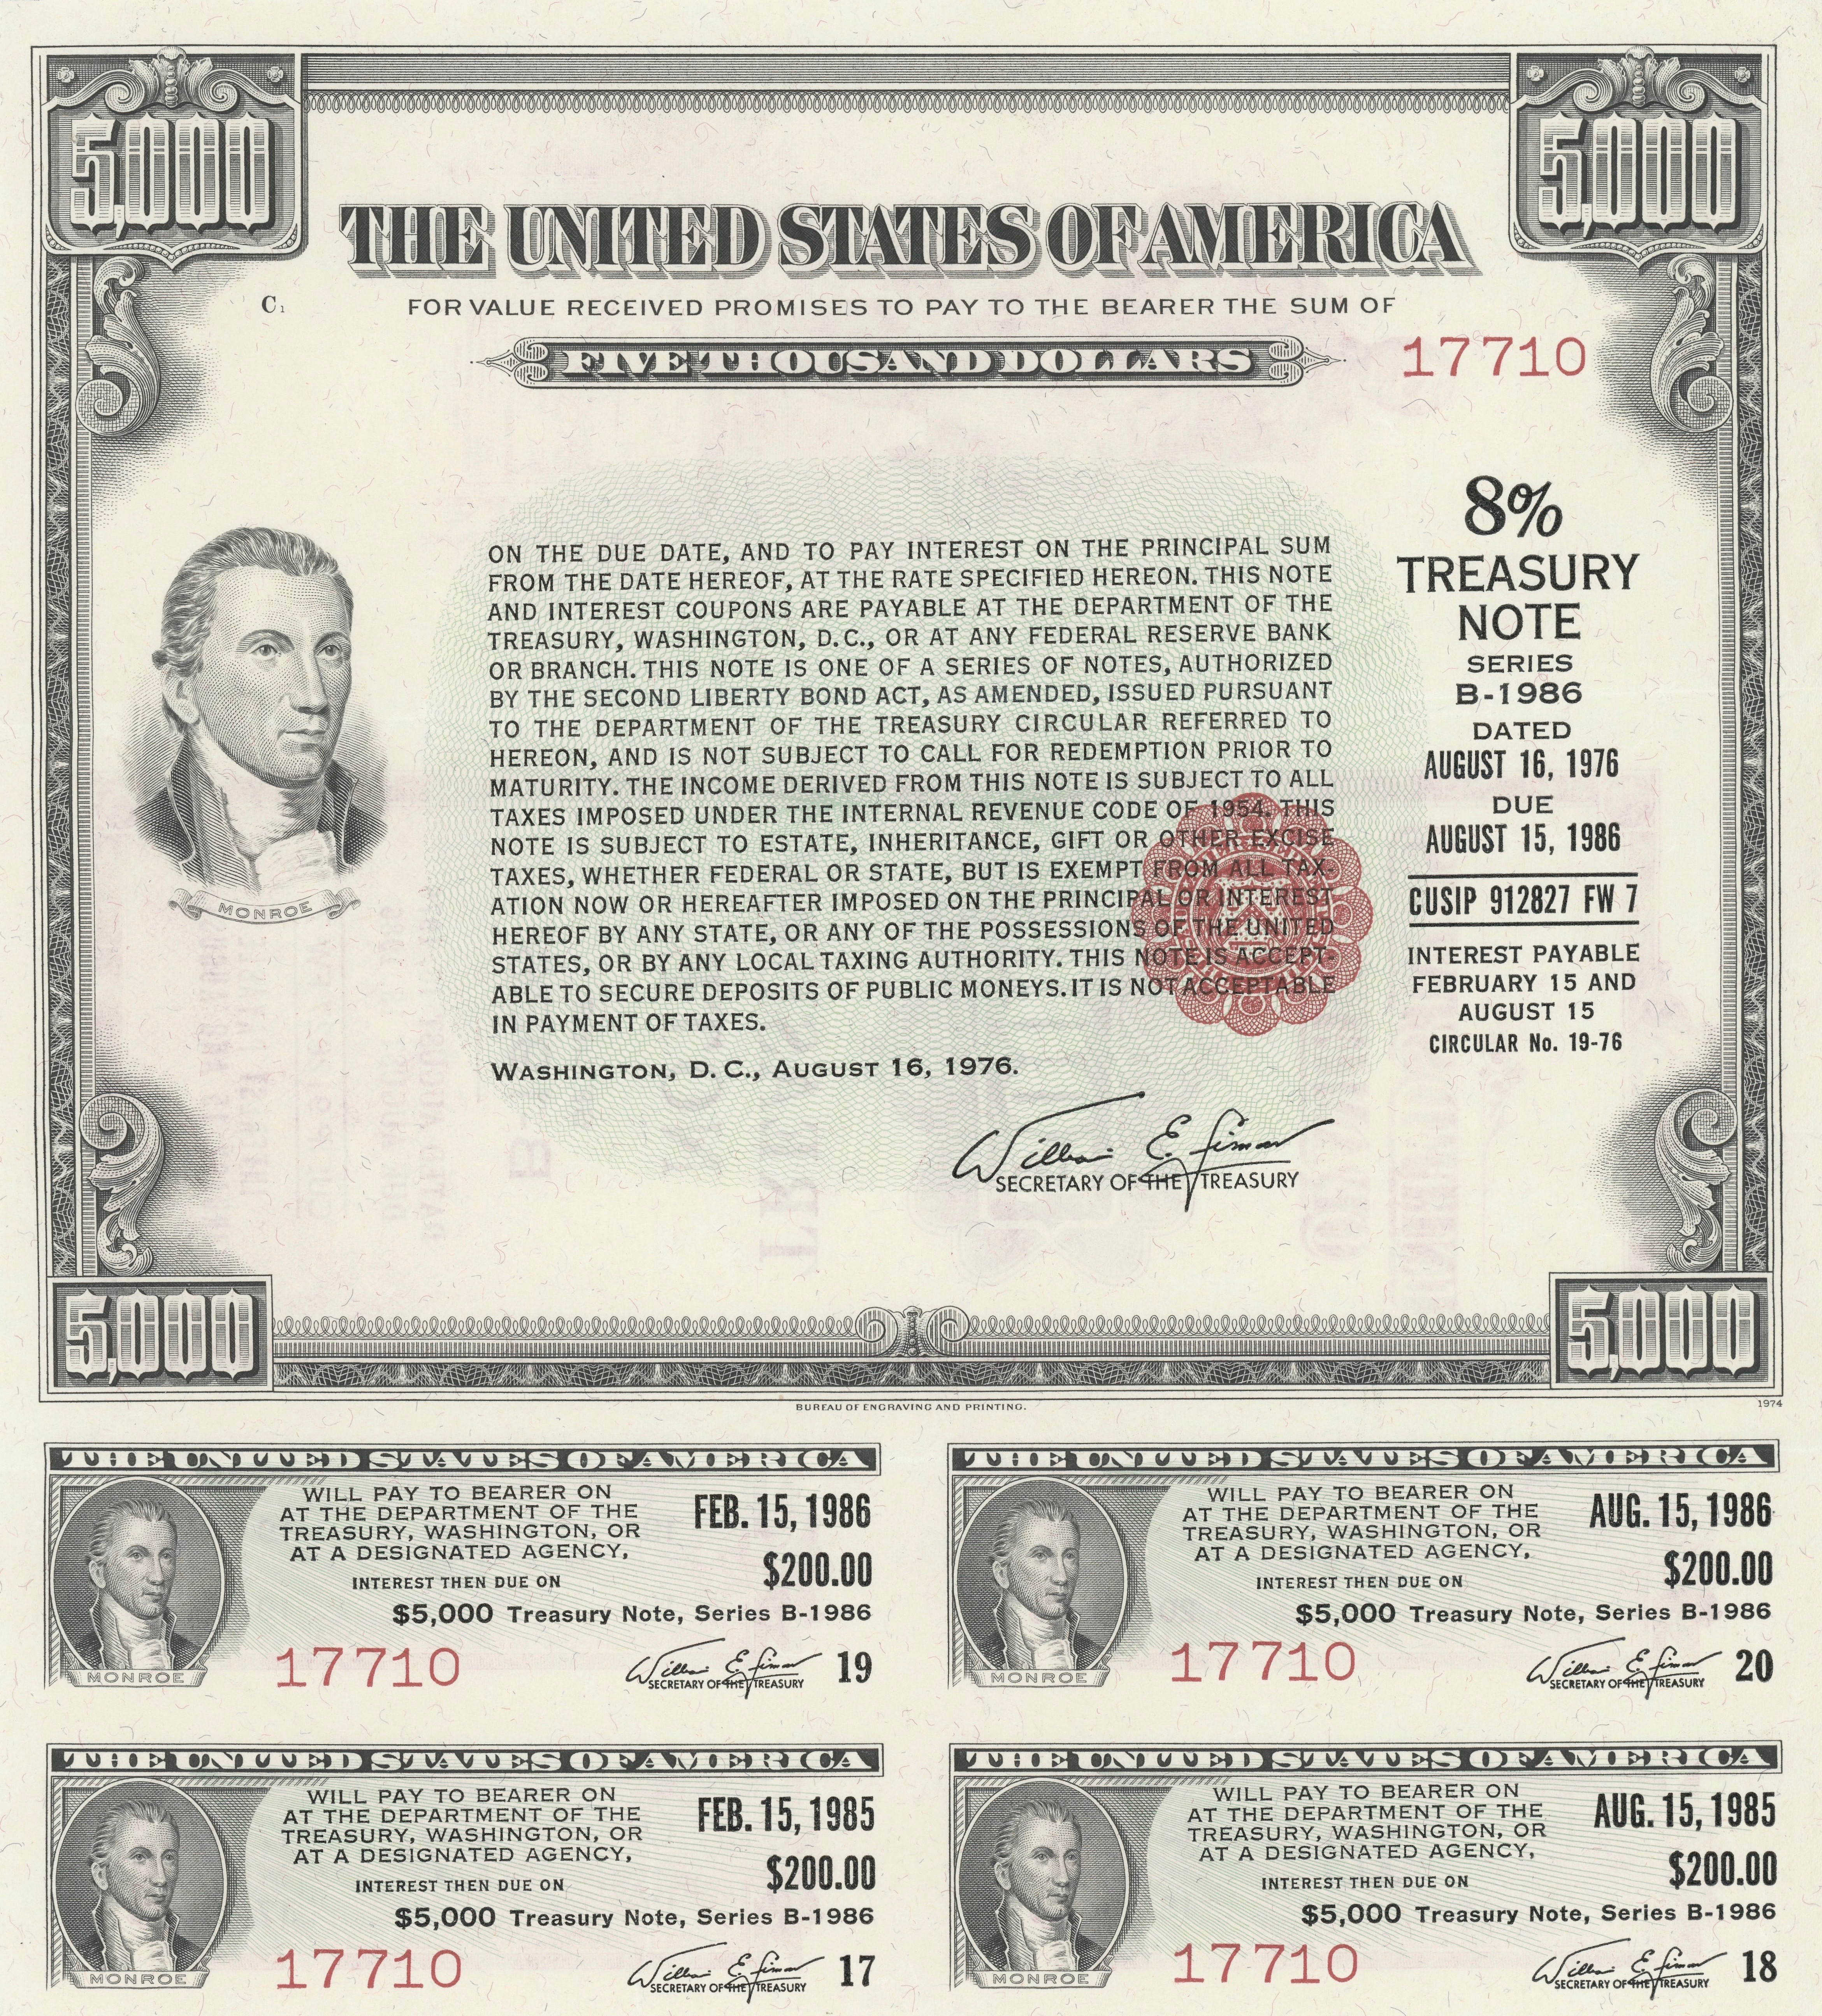
\includegraphics[width=0.5\textwidth]{figures/intro_b_fig3.png}

    \blfootnote{Source: The Joe I. Herbstman Memorial Collection of American Finance}

\end{frame}

\begin{frame}[t]
    \frametitle{3. Income}
    \framesubtitle{Timing of Income}

    Be careful with the timing of income.   
    Often a problem will say "you purchase a stock that just paid a dividend." 
    Do NOT count that dividend in the total return.
    \vspace{1em}

    \centering
    \includegraphics[width=1\textwidth]{figures/ch5_1_timeline.png}

\end{frame}

\begin{frame}[t]
    \frametitle{3. Income}
    \framesubtitle{Example: AAPL}

    \vspace{-1em}
    \begin{columns}
        \begin{column}{0.48\textwidth}
            \centering
            \begin{table}
            \caption{AAPL Dividends in 2024}
                \begin{tabular}{lr}
                    \toprule
                    date & dividend \\
                    \midrule
                    2024-02-09 & 0.24 \\
                    2024-05-10 & 0.25 \\
                    2024-08-12 & 0.25 \\
                    2024-11-08 & 0.25 \\
                    \bottomrule
                \end{tabular}
            \end{table}
        \end{column}

        \begin{column}{0.48\textwidth}
            \centering
            \includegraphics[width=\textwidth]{figures/ch5_1_appl_wincome.png}
        \end{column}
    \end{columns}
    \vspace{1em}

    The price of AAPL was 185.64 on January 2, 2024.   
    The price of AAPL rose to 250.42 on December 31, 2024.  
    What was the Holding Period Return from owning AAPL stock throughout 2024?

    \blfootnote{Data source: Yahoo finance}

\end{frame}

\begin{frame}[t]
    \frametitle{3. Income}
    \framesubtitle{Example: S\&P Total Return}

    \centering
    \includegraphics[width=0.8\textwidth]{figures/ch5_1_sp500_tr.png}

    \blfootnote{Data source: Interactive Brokers (SPX and SPXT)}

\end{frame}

\begin{frame}[t]
    \frametitle{4. Measurement Issues}
    \framesubtitle{Compounding: APR}

    Annual Percentage Rates of Return\\
    $$(1 + \text{EAR}) = \left(1+\frac{APR}{n}\right)^n$$\\
    $$\text{APR} = n \times [(1+\text{EAR})^{1/n} - 1]$$

    \begin{itemize}
        \item Where $n$ is the number of compounding periods per year\\
        \item After calculating the rate ($\frac{APR}{n}$) then compound to get annual rate\\
        \item This is the convention used in short term investments\\
        \item Bonds typically have semi annual compounding (2 times per year), and the coupon
        is given by $\frac{\text{Coupon Rate}}{2}$
    \end{itemize}

\end{frame}

\begin{frame}[t]
    \frametitle{4. Measurement Issues}
    \framesubtitle{Compounding: Definition of e}

        The exponential function $e^x$ can be defined as a limit:
    \[
        e^x = \lim_{n \to \infty} \left(1 + \frac{x}{n}\right)^n
    \]
    Notice the similarity to the formula for the APR.\\
    \vspace{1em}
    As $n \to \infty$ the formula for the $APR \to e^{r_{cc}}$, 
    where $r_{cc}$ is the "continuously compounded" rate of return.

\end{frame}    

\begin{frame}[t]
    \frametitle{4. Measurement Issues}
    \framesubtitle{Compounding}

    Continuously compounded rate of return $(r_{cc})$:
    $$1 + \text{EAR} = exp(r_{cc}) = e^{r_{cc}}$$
    
    \begin{itemize}
        \item If you are given $e^{r_{cc}}$, then with a little rearranging you can find $EAR$: $\text{EAR} = e^{r_{cc}} - 1$
        \item Conversely, if you are given $EAR$ then you can take $ln()$ of both sides to find $r_{cc}$
    \end{itemize}
    \vspace{1em}

    Most of the time in Econ 457 the compounding is either annual, or at the same frequency as the income (e.g. coupons, dividends).  
    Occassionally we'll use continous compounding makes the math easier (e.g. option pricing).

\end{frame}

\begin{frame}[t]
    \frametitle{4. Measurement Issues}
    \framesubtitle{Compounding: Log scale}

    \begin{columns}
        \begin{column}{0.55\textwidth}
            \centering
            \includegraphics[width=\textwidth]{figures/ch5_1_sp500.png}
        \end{column}
        \begin{column}{0.55\textwidth}
            \centering
            \includegraphics[width=\textwidth]{figures/ch5_1_sp500_logscale.png}
        \end{column}
    \end{columns}

    \blfootnote{\raggedright Data Source: Robert Shiller, www.shillerdata.com}

\end{frame}

\begin{frame}[t]
    \frametitle{4. Measurment Issues}
    \framesubtitle{Compounding: Reinvestment}
    What did you do with the income?   The initial expression for HPR assumed you did nothing.\\
    \vspace{1em}
    The expressions for EAR and APR assumed income was reinvested regularly.\\
    \vspace{1em}
    The correct choice depends on the context.  It's easy to reinvest income from an ETF, it may be harder in a privately held stock.

\end{frame}

\begin{frame}[t]
    \frametitle{4. Measuring returns}
    \framesubtitle{Geometric v. Arithmetic Mean}

    For a series of returns, the \textit{arithmetic} average is:
    $$r_{ave} = \frac{1}{T}\times\sum_{i=1}^{T}(1 + r_i)$$

    The \textit{geometric} average is:
    $$r_{geo-ave} = \sqrt[T]{\prod_{i=1}^{T} (1 + r_i)}$$

\end{frame}

\begin{frame}[t]
    \frametitle{4. Measuring returns}
    \framesubtitle{Geometric v. Arithmetic Mean}

    The arithmetic average is \underline{always greater} than the geometric average.\\
    \vspace{1em}
    You can show this using the fact that the $ln()$ function is concave (next slide).\\
    
    \vspace{1em}
    The difference between the arithmetic and geometric averages is increasing in the variance of the return series.

\end{frame}

\begin{frame}[t]
    \frametitle{4. Measuring returns}
    \framesubtitle{Geometric v. Arithmetic Mean}

    \footnotesize
    Showing that the Geometric Mean $<$ the Arithmetic Mean
    \begin{align}
        \text{Geometric Mean} = \sqrt[T]{\prod_{i=1}^{T} x_i}\\
        \ln(\text{Geometric Mean}) = \frac{1}{T} \sum_{i=1}^{T} \ln(x_i)\\
        < \ln\left(\frac{1}{T} \sum_{i=1}^{T} (x_i)\right)\\
        < \ln(\text{Arithmetic Mean})\\
        \implies \text{Geometric Mean} < \text{Arithmetic Mean}
    \end{align}
    Where (2) applies properties of $ln()$, (3) is because $ln()$ is a concave function 
    (Jensen's inequality), and (4) is because $ln()$ is monotonically increasing.

\end{frame}

\begin{frame}[t]
    \frametitle{4. Measuring returns}
    \framesubtitle{Geometric v. Arithmetic Mean, Example}

    Stock ABC doesn't pay dividends.   In year 1 the price of ABC declines by 20\%.   
    In year 2 the price rebounds by 20\%.\\ 
    \vspace{1em} 
    What is the arithmetic average of the annual returns?   What is the geometric average?
    \vspace{1em}
    Which measure is more appropriate?

\end{frame}

\begin{frame}[t]
    \frametitle{4. Measurement Issues}
    \framesubtitle{Total Return Series}

    A total return series reflects the growth of an investment due to both price changes and income.\\
    \vspace{1em}
    The convention is to incorporate the income in the period that it is received.   
    This is most appropriate for monthly series.   May consider alternatives for a daily series.\\
    \vspace{1em}
    Bonds have a different convention, which we will discuss later.

\end{frame}

\begin{frame}[t]
    \frametitle{4. Measurement Issues}
    \framesubtitle{Total Return Series}

    Constructing a total return index:
    \begin{enumerate}
      \item Start: 
      $$index_{t0} = 100$$
      \item Calculate holding period return: 
      $$\text{HPR}_{t1} = \frac{(\text{income} + \text{price change})}{\text{Initial Price}}-1$$
      \item The value for the next period is given by: 
      $$index_{t+1} = (1+\text{HPR}_{t1}) \cdot index_{t}$$
      \item Repeat...
    \end{enumerate}

\end{frame}

{
\setbeamertemplate{footline}{}
\begin{frame}[t]
    \frametitle{4. Measurement Issues}
    \framesubtitle{Total Return Series, Arthmetic v. Geometric Mean}
    
    \vspace{-1em}
    \scriptsize
    \begin{table}
    \caption{S\&P 500 Total Returns by Decade, (\% Annualized)}
    \begin{tabular}{lrrr}
    \toprule
    Decade & Arithmetic Return & Geometric Mean & Standard Deviation \\
    \midrule
    1870s & 8.11 & 7.46 & 10.86 \\
    1880s & 6.29 & 5.83 & 9.62 \\
    1890s & 6.24 & 5.55 & 11.84 \\
    1900s & 10.62 & 9.82 & 12.70 \\
    1910s & 4.99 & 4.44 & 10.51 \\
    1920s & 15.46 & 14.25 & 15.08 \\
    1930s & 4.39 & 0.03 & 30.63 \\
    1940s & 9.47 & 8.58 & 13.23 \\
    1950s & 18.24 & 17.74 & 10.08 \\
    1960s & 8.05 & 7.51 & 10.31 \\
    1970s & 6.56 & 5.69 & 13.23 \\
    1980s & 16.88 & 16.04 & 12.98 \\
    1990s & 17.19 & 16.66 & 10.45 \\
    2000s & 0.38 & -0.73 & 14.68 \\
    2010s & 13.02 & 12.56 & 9.55 \\
    2020s & 13.72 & 12.11 & 14.15 \\
    \bottomrule
    \end{tabular}
    \end{table}

    \blfootnote{Data Source: Robert Shiller, Ken French.  Monthly data annualized.}

\end{frame}
}

\begin{practiceframe}[t]
    \frametitle{5. Excel}
    \framesubtitle{Some basic commands}

    vlookup(): Used to match data from different tabs\\
    \vspace{1em}

    isna(): Tell Excel how to treat missing values\\
    \vspace{1em}

    \$: Used to 'freeze' the cell row or column
    \vspace{1em}

    Excel dates: can change the format
    \vspace{1em}

    Charts: mostly use line chart in this class
    \vspace{1em}

\end{practiceframe}

\end{document}